\section{Entradas y salidas del sistema}
\sectionmark{Entradas y salidas}

El Synthi 100 posee una serie de entradas y salidas de audio que permiten la recepción y el envío de señales. En la aplicación se ha procedido de un modo análogo al sintetizador, aprovechando la capacidad de SuperCollider de crear cualquier cantidad de puertos desde el servidor de sonido, quedando a disposición del sistema operativo. Estos canales pueden recibir audio --en este caso siempre digital-- y enviar audio desde y hacia cualquier otro software instalado. SuperCollider nombra automáticamente estos puertos numerándolos. La tabla \ref{table:inputs_outputs} muestra la correspondencia entre estos y los del Synthi. 

\begin{table}
	\begin{center}
		\begin{tabular}{|l|l|l|l| }
			\hline
			\multirow{4}{*}{\parbox{5em}{Pan\\ outputs}} & \multirow{2}{*}{\parbox{5em}{  Channels\\ 1--4}} 
			 & Left & \texttt{SuperCollider:out\_3}\\			
			 & & Right & \texttt{SuperCollider:out\_4}\\	
			 \cline{2-4}
			 & \multirow{2}{*}{\parbox{5em}{  Channels\\ 5--8}} 
			 & Left & \texttt{SuperCollider:out\_5}\\	
			 & & Right & \texttt{SuperCollider:out\_6}\\			
			 \hline
			 \hline
			 \multirow{8}{*}{} & \multirow{8}{*}{ \parbox{5em}{ Individual\\ channels\\ outputs}}
			 & 1 & \texttt{SuperCollider:out\_7}\\			
			 & & 2 & \texttt{SuperCollider:out\_8}\\			
			 & & 3 & \texttt{SuperCollider:out\_9}\\			
			 & & 4 & \texttt{SuperCollider:out\_10}\\			
			 & & 5 & \texttt{SuperCollider:out\_11}\\			
			 & & 6 & \texttt{SuperCollider:out\_12}\\			
			 & & 7 & \texttt{SuperCollider:out\_13}\\			
			 & & 8 & \texttt{SuperCollider:out\_14}\\			
			 \hline
			 \hline
			 \multirow{8}{*}{\parbox{5em}{External\\ treatment\\ devices}} &  \multirow{4}{*}{\parbox{5em}{  Send\\ to device}}
			 & 1 & \texttt{SuperCollider:out\_15}\\			
			 & & 2 & \texttt{SuperCollider:out\_16}\\			
			 & & 3 & \texttt{SuperCollider:out\_17}\\			
			 & & 4 & \texttt{SuperCollider:out\_18}\\			
			 \cline{2-4}
			 & \multirow{4}{*}{\parbox{5em}{  Return from device}}
			 & 1 & \texttt{SuperCollider:in\_3}\\			
			 & & 2 & \texttt{SuperCollider:in\_4}\\			
			 & & 3 & \texttt{SuperCollider:in\_5}\\			
			 & & 4 & \texttt{SuperCollider:in\_6}\\			
			 \hline
			 \hline
			\multirow{8}{*}{} &  \multirow{8}{*}{\parbox{5em}{  Input\\ amplifiers}}
			 & 1 & \texttt{SuperCollider:in\_7}\\			
			 & & 2 & \texttt{SuperCollider:in\_8}\\			
			 & & 3 & \texttt{SuperCollider:in\_9}\\			
			 & & 4 & \texttt{SuperCollider:in\_10}\\			
			 & & 5 & \texttt{SuperCollider:in\_11}\\			
			 & & 6 & \texttt{SuperCollider:in\_12}\\			
			 & & 7 & \texttt{SuperCollider:in\_13}\\			
			 & & 8 & \texttt{SuperCollider:in\_14}\\		
			\cline{2-4}
			 \multirow{2}{*}{} &  \multirow{2}{*}{Mic amp}
			 & 1 & \texttt{SuperCollider:in\_15}\\			
			 & & 2 & \texttt{SuperCollider:in\_16}\\			
			 \hline
		\end{tabular}
		\caption[Entradas y salidas de la aplicación]{Entradas y salidas de audio del Synthi 100 y su correspondencia con las de la aplicación.}
		\label{table:inputs_outputs}
	\end{center}
\end{table}

Como se puede observar, se han reservado las dos primeras entradas y las dos primeras salidas para el propio sistema operativo. Por defecto, SuperCollider conecta las entradas 1 y 2 al micrófono del sistema y las salidas 1 y 2 a los altavoces (Ver \ref{fig:entradas_salidas}). Dependiendo del sistema operativo o del software controlador del audio utilizado, los puertos pueden ser renombrados para ser utilizados de forma más intuitiva. 

\begin{figure}
	\centering
	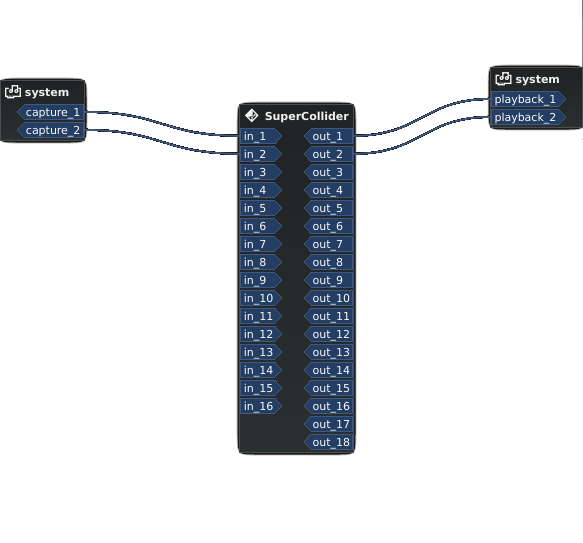
\includegraphics[width=0.7\textwidth]{images/entradas_salidas}
	\caption[Entradas y salidas al sistema]{Entradas y salidas de SuperCollider al sistema operativo con \appName. Los dos primeros puertos de entrada y de salida, están reservados por defecto a la entrada y salida estandar (micrófono y altavoces del ordenador).. Los puertos están numerados, y respetan el mismo orden que el que se encuentra en el Synthi 100}
	\label{fig:entradas_salidas}
\end{figure}

Cabe destacar, entre las salidas, dos estereofónicas que combinan varios canales de salida, \textit{Pan Outputs}. Una combina a los canales del 1 al 4, mientras que la segunda los del 5 al 8. Estos canales, como se verá en su sección (\ref*{sec:output_channels}), tienen un dial para panear la señal. Esto solo tiene efecto en estos puertos combinados.